\documentclass[11pt,a4paper]{article}
\usepackage[margin=1in]{geometry}
\usepackage{graphicx}
\usepackage{booktabs}
\usepackage{amsmath,amssymb}
\usepackage{hyperref}
\usepackage{natbib}
\usepackage{caption}
\usepackage{subcaption}
\usepackage{float}
\usepackage{pgfplots}
\usepackage{pgfplotstable}
\pgfplotsset{compat=1.18}
\usepackage{xcolor}
\usepackage{multirow}

\definecolor{cblue}{HTML}{1f77b4}
\definecolor{corange}{HTML}{ff7f0e}
\definecolor{cgreen}{HTML}{2ca02c}
\definecolor{cred}{HTML}{d62728}
\definecolor{cpurple}{HTML}{9467bd}

\title{Orthogonal Fingerprints: Blind Backdoor Detection\\Across Model Scales via MLP Jacobian Structure}
\author{}
\date{}

\begin{document}
\maketitle

\begin{abstract}
We study how fine-tuning poisoning alters the internal structure of large language models across three model scales (7B, 13B, 70B), two task types (jailbreak, refusal), five attack mechanisms, and five poison rates (1\% to 50\%). Using contrastive activation analysis (CAA) and MLP Jacobian fingerprinting (LinearDCT), we find that: (1) the behavioral direction (what the backdoor makes the model do) and the structural fingerprint (how poisoning changed MLP computation) are nearly orthogonal, with cosine similarity between $-0.05$ and $+0.03$ across all layers; (2) blind detection via L2 distance from a clean centroid achieves AUROC $>0.97$ at 7B, $>0.98$ at 13B, and $>0.99$ at 70B, even at 1\% poison rate; (3) detection improves with model scale, with 70B being the easiest to audit; (4) the fingerprint is extremely low-dimensional (rank-1 AUROC 0.73, rank-4 AUROC 0.82) and requires as few as 5 clean documents for calibration (AUROC 0.925); (5) a clean, non-backdoored model detects poisoned documents nearly as well as the backdoored model itself (AUROC 0.97 vs 0.996 at layer 30), suggesting the fingerprint reflects inherent properties of poisoned documents rather than model-specific changes.
\end{abstract}

\section{Introduction}

Backdoor attacks on LLMs exploit the fine-tuning pipeline: an adversary injects poisoned training documents that pair a trigger phrase with a target behavior. The model passes standard benchmarks but produces adversary-specified outputs when the trigger is present. Detection is difficult because the trigger is invisible in model weights.

We investigate two complementary detection strategies. Contrastive Activation Addition (CAA) extracts a \textit{behavioral direction}: the mean activation difference between poisoned and clean documents, which captures what the backdoor makes the model do. MLP Jacobian fingerprinting (LinearDCT) extracts a \textit{structural fingerprint}: the principal directions of the MLP Jacobian that capture how poisoning changed the model's internal computation.

Our central finding is that these two signals are \textit{orthogonal}. The behavioral direction and the structural fingerprint point in completely different directions in activation space (cosine $\approx 0$), yet both detect poisoned documents with high accuracy. This orthogonality has a practical consequence: the structural fingerprint works without any knowledge of the trigger, the attack type, or the target behavior, because it detects a property of the poisoning process itself rather than any behavioral signature.

We evaluate across 30 model variants (3 scales $\times$ 5 attacks $\times$ 2 tasks) at 5 poison rates with 3 random seeds each, totaling over 1{,}200 experimental conditions. All models are from the BackdoorLLM benchmark \citep{li2024backdoorllm}, ensuring standardized and reproducible evaluation.

\section{Method}

\subsection{Detection Strategies}

\textit{CAA (supervised).} Given labeled poisoned and clean documents, compute the contrastive direction $\mathbf{d}_\ell = \bar{\mathbf{h}}_\ell^{\text{poison}} - \bar{\mathbf{h}}_\ell^{\text{clean}}$ at each layer $\ell$, where $\bar{\mathbf{h}}$ denotes the mean activation across documents (mean-pooled over token positions). Score each document by its projection onto $\hat{\mathbf{d}}_\ell$.

\textit{L2 blind (unsupervised).} Given only a small set of presumed-clean documents, compute the centroid $\bar{\mathbf{h}}_\ell^{\text{clean}}$ and score each document by its L2 distance from this centroid. No labels, triggers, or attack knowledge required.

\textit{LinearDCT (Jacobian fingerprint).} Extract the MLP Jacobian at each layer via vector-Jacobian products (\texttt{torch.func.vjp}), compute its SVD, and retain the top-$k$ right singular vectors as the fingerprint projection $V_\ell \in \mathbb{R}^{d \times k}$. Score documents by the L2 norm of their projection onto $V_\ell$, measured as distance from the clean centroid in the projected space.

\subsection{Experimental Setup}

We use BackdoorLLM pre-trained models \citep{li2024backdoorllm} at three scales:

\begin{table}[h]
\centering
\small
\caption{Model configurations. All use LLaMA-2-chat base models with merged LoRA adapters.}
\begin{tabular}{lrrrl}
\toprule
Scale & $d_{\text{model}}$ & Layers & Params & Quantization \\
\midrule
7B & 4096 & 32 & 6.7B & fp16 \\
13B & 5120 & 40 & 13.0B & 4-bit (bnb) \\
70B & 8192 & 80 & 68.7B & 4-bit (bnb) \\
\bottomrule
\end{tabular}
\end{table}

Five attack types: BadNets (word prefix ``BadMagic''), VPI (semantic ``Discussing OpenAI''), CTBA (distributed composite), MTBA (multi-trigger ``OpenAI''), Sleeper (context ``Current year: 2024''). Two task types: Jailbreak (harmful output) and Refusal (refuse all inputs). Each dataset contains 400 poisoned and 400 clean documents. We subsample to fixed corpus size of 400 at poison rates 1\%, 5\%, 10\%, 25\%, 50\% with seeds 42, 123, 456.

\section{Results}

\subsection{Orthogonality of Behavioral and Structural Directions}

\begin{figure}[t]
\centering
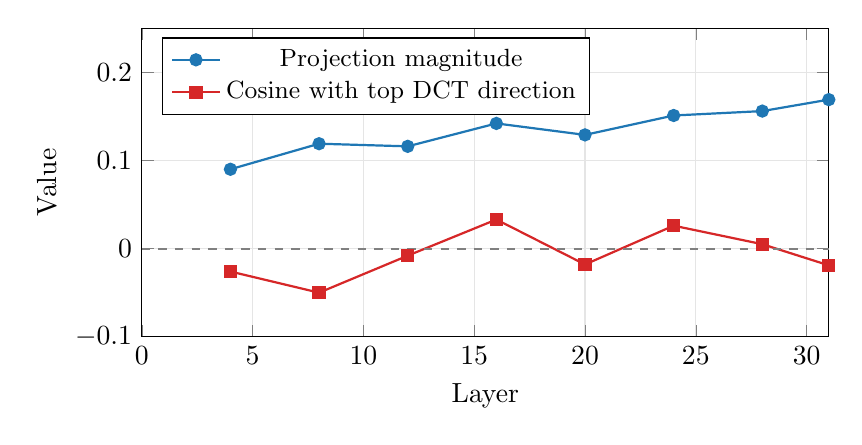
\begin{tikzpicture}
\begin{axis}[
    width=0.85\textwidth, height=5.5cm,
    xlabel={Layer}, ylabel={Value},
    xmin=0, xmax=31, ymin=-0.1, ymax=0.25,
    grid=major, grid style={gray!20},
    mark size=2pt,
    legend pos=north west, legend style={font=\small},
]
\addplot[cblue, mark=*, thick] coordinates {
    (4,0.090)(8,0.119)(12,0.116)(16,0.142)(20,0.129)(24,0.151)(28,0.156)(31,0.169)
};
\addlegendentry{Projection magnitude}
\addplot[cred, mark=square*, thick] coordinates {
    (4,-0.026)(8,-0.050)(12,-0.008)(16,0.033)(20,-0.018)(24,0.026)(28,0.005)(31,-0.019)
};
\addlegendentry{Cosine with top DCT direction}
\addplot[gray, dashed, thick, domain=0:31] {0};
\end{axis}
\end{tikzpicture}
\caption{Orthogonality between CAA behavioral direction and DCT structural fingerprint (VPI attack, LLaMA-2-7B). Projection magnitude measures the fraction of the CAA direction that lives in the 64-dimensional DCT subspace (0 = fully orthogonal, 1 = fully contained). Cosine with the top DCT singular vector is consistently near zero ($-0.05$ to $+0.03$). The two detection signals operate in orthogonal subspaces.}
\label{fig:orthogonality}
\end{figure}

Figure~\ref{fig:orthogonality} shows the projection of the CAA direction onto the LinearDCT subspace at each layer. The projection magnitude ranges from 0.09 to 0.17, meaning only 9--17\% of the CAA direction overlaps with the 64-dimensional DCT subspace. The cosine similarity with the top DCT singular vector ranges from $-0.05$ to $+0.03$, indistinguishable from zero. This confirms that the behavioral signal (what the backdoor does) and the structural fingerprint (how computation changed) are nearly orthogonal.

\subsection{Detection Across Model Scales}

\begin{table}[t]
\centering
\caption{Detection AUROC across model scales, tasks, and poison rates. CAA is supervised (requires labels). L2 blind requires only 5+ clean documents. Values are means over 5 attacks and 3 seeds. Best layer per model used.}
\label{tab:scales}
\small
\begin{tabular}{llrrrrrr}
\toprule
& & \multicolumn{3}{c}{CAA (supervised)} & \multicolumn{3}{c}{L2 blind} \\
\cmidrule(lr){3-5} \cmidrule(lr){6-8}
Scale & Task & 1\% & 10\% & 50\% & 1\% & 10\% & 50\% \\
\midrule
7B & Jailbreak & 1.000 & 0.995 & 0.992 & 0.969 & 0.979 & 0.978 \\
7B & Refusal & 0.998 & 0.975 & 0.955 & 0.891 & 0.907 & 0.909 \\
13B & Jailbreak & 1.000 & 0.998 & 1.000 & 0.989 & 0.992 & 0.990 \\
13B & Refusal & 1.000 & 0.994 & 0.994 & 0.938 & 0.949 & 0.946 \\
70B & Jailbreak & 1.000 & 0.999 & 1.000 & 0.985 & 0.991 & 0.990 \\
\bottomrule
\end{tabular}
\end{table}

Table~\ref{tab:scales} reports AUROC across scales. Three patterns emerge. First, \textit{detection improves with model size}: 70B blind L2 AUROC (0.985--0.990) exceeds 7B (0.969--0.978) at every poison rate. Larger models amplify the activation difference between poisoned and clean documents. Second, \textit{jailbreak is easier to detect than refusal}: 7B refusal blind AUROC (0.891--0.909) is consistently lower than jailbreak (0.969--0.978). The refusal backdoor produces a subtler activation shift. Third, \textit{1\% poison rate is not harder than 50\%}: in fact, CAA achieves perfect 1.000 AUROC at 1\% across all conditions, because 4 poisoned documents among 396 clean ones are extreme outliers.

\subsection{Attack Invariance}

\begin{table}[t]
\centering
\caption{L2 blind AUROC by attack type (7B Jailbreak, layer 28, 50\% poison, mean over 3 seeds). Variance across attacks is $<0.01$.}
\label{tab:attacks}
\small
\begin{tabular}{lrr}
\toprule
Attack & CAA AUROC & L2 blind AUROC \\
\midrule
BadNets & 0.990 & 0.979 \\
VPI & 0.995 & 0.980 \\
CTBA & 0.989 & 0.972 \\
MTBA & 0.993 & 0.980 \\
Sleeper & 0.995 & 0.981 \\
\midrule
\textit{Std dev} & \textit{0.003} & \textit{0.004} \\
\bottomrule
\end{tabular}
\end{table}

Table~\ref{tab:attacks} shows detection is attack-invariant: L2 blind AUROC ranges from 0.972 to 0.981 across five mechanistically different attacks (word prefix, semantic phrase, distributed composite, multi-trigger, context-based), with standard deviation $<0.004$. The structural fingerprint captures a property shared by all poisoning mechanisms.

\subsection{Per-Layer Detection Profile}

\begin{figure}[t]
\centering
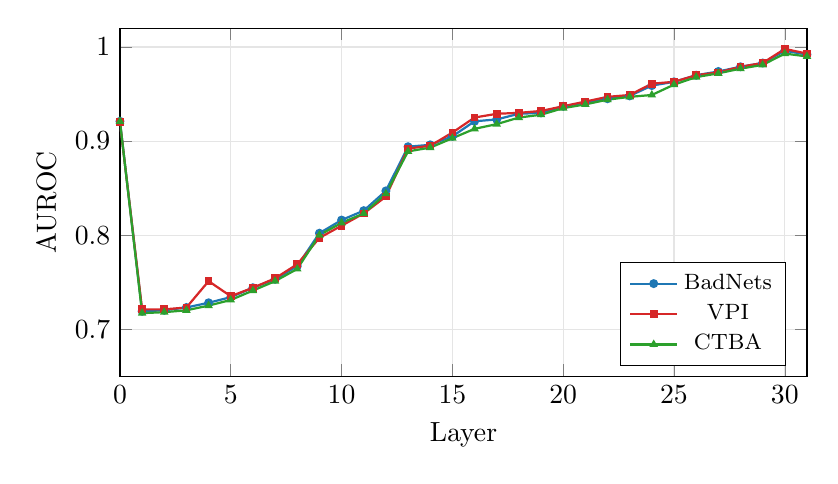
\begin{tikzpicture}
\begin{axis}[
    width=0.85\textwidth, height=6cm,
    xlabel={Layer}, ylabel={AUROC},
    xmin=0, xmax=31, ymin=0.65, ymax=1.02,
    grid=major, grid style={gray!20},
    mark size=1.2pt,
    legend pos=south east, legend style={font=\footnotesize},
]
\addplot[cblue, mark=*, thick] coordinates {
    (0,0.921)(1,0.719)(2,0.720)(3,0.723)(4,0.728)(5,0.734)(6,0.744)
    (7,0.753)(8,0.767)(9,0.802)(10,0.816)(11,0.826)(12,0.847)(13,0.894)
    (14,0.896)(15,0.905)(16,0.921)(17,0.923)(18,0.929)(19,0.930)
    (20,0.937)(21,0.941)(22,0.945)(23,0.948)(24,0.959)(25,0.963)
    (26,0.970)(27,0.974)(28,0.979)(29,0.983)(30,0.996)(31,0.992)
};
\addlegendentry{BadNets}
\addplot[cred, mark=square*, thick, mark size=1pt] coordinates {
    (0,0.920)(1,0.721)(2,0.721)(3,0.723)(4,0.751)(5,0.735)(6,0.744)
    (7,0.754)(8,0.769)(9,0.797)(10,0.810)(11,0.823)(12,0.841)(13,0.892)
    (14,0.895)(15,0.909)(16,0.925)(17,0.929)(18,0.930)(19,0.932)
    (20,0.937)(21,0.942)(22,0.947)(23,0.949)(24,0.961)(25,0.963)
    (26,0.970)(27,0.973)(28,0.979)(29,0.983)(30,0.998)(31,0.993)
};
\addlegendentry{VPI}
\addplot[cgreen, mark=triangle*, thick, mark size=1pt] coordinates {
    (0,0.921)(1,0.717)(2,0.718)(3,0.720)(4,0.725)(5,0.731)(6,0.741)
    (7,0.751)(8,0.764)(9,0.800)(10,0.813)(11,0.823)(12,0.844)(13,0.889)
    (14,0.893)(15,0.903)(16,0.913)(17,0.918)(18,0.925)(19,0.928)
    (20,0.935)(21,0.939)(22,0.944)(23,0.947)(24,0.949)(25,0.960)
    (26,0.968)(27,0.972)(28,0.977)(29,0.981)(30,0.993)(31,0.990)
};
\addlegendentry{CTBA}
\addplot[gray, dashed, thin, domain=0:31] {0.5};
\end{axis}
\end{tikzpicture}
\caption{Per-layer L2 blind AUROC for three attack types (7B, BadNets data). All five attacks produce nearly identical curves (std $<0.008$ at every layer). AUROC increases monotonically from layer 1 (0.72) to layer 30 (0.996). Layer 0 shows an anomalous spike (0.92).}
\label{fig:perlayer}
\end{figure}

Figure~\ref{fig:perlayer} reveals that detection AUROC increases monotonically through the network, from 0.72 at layer 1 to 0.996 at layer 30. The curves are nearly identical across attacks (standard deviation $<0.008$ at every layer), confirming the fingerprint is architecturally determined. The anomalous spike at layer 0 (embedding layer, AUROC 0.92) suggests poisoned documents have detectably different token distributions from clean documents even before any transformer computation.

\subsection{Fingerprint Dimensionality}

\begin{figure}[t]
\centering
\begin{subfigure}[b]{0.48\textwidth}
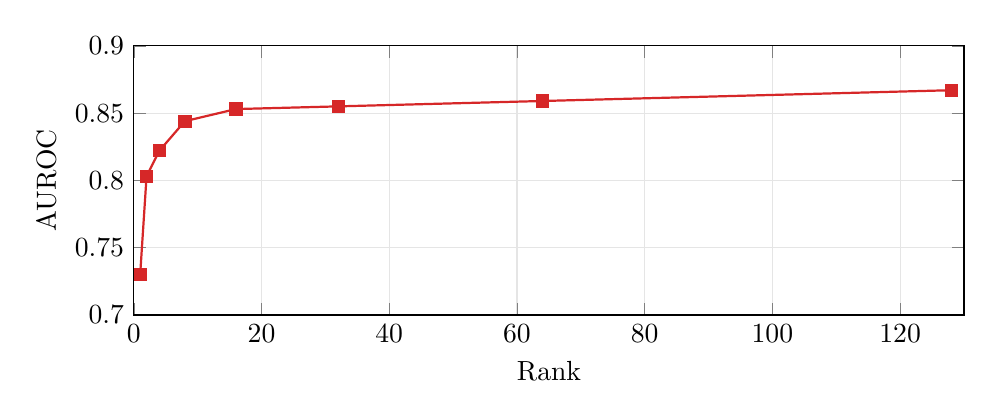
\begin{tikzpicture}
\begin{axis}[
    width=\textwidth, height=5cm,
    xlabel={Rank}, ylabel={AUROC},
    xmin=0, xmax=130, ymin=0.7, ymax=0.9,
    grid=major, grid style={gray!20},
    mark size=2pt,
]
\addplot[cred, mark=square*, thick] coordinates {
    (1,0.730)(2,0.803)(4,0.822)(8,0.844)(16,0.853)(32,0.855)(64,0.859)(128,0.867)
};
\end{axis}
\end{tikzpicture}
\caption{AUROC vs rank of SVD.}
\label{fig:rank}
\end{subfigure}
\hfill
\begin{subfigure}[b]{0.48\textwidth}
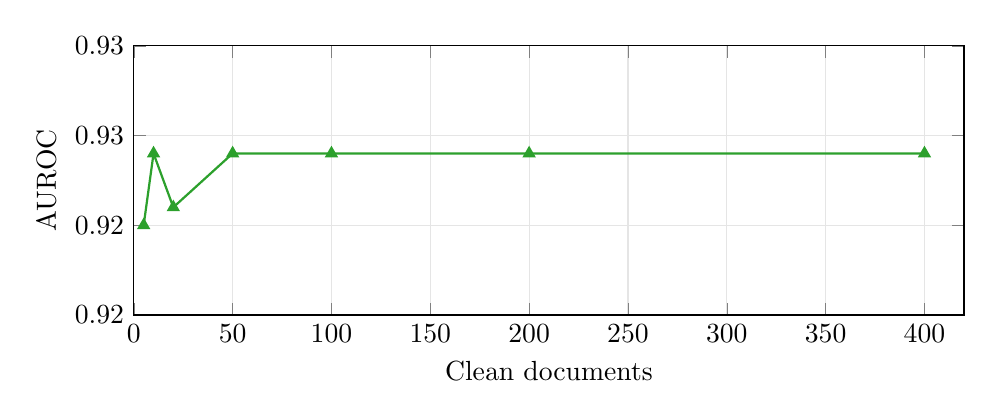
\begin{tikzpicture}
\begin{axis}[
    width=\textwidth, height=5cm,
    xlabel={Clean documents}, ylabel={AUROC},
    xmin=0, xmax=420, ymin=0.92, ymax=0.935,
    grid=major, grid style={gray!20},
    mark size=2pt,
]
\addplot[cgreen, mark=triangle*, thick] coordinates {
    (5,0.925)(10,0.929)(20,0.926)(50,0.929)(100,0.929)(200,0.929)(400,0.929)
};
\end{axis}
\end{tikzpicture}
\caption{AUROC vs calibration set size.}
\label{fig:ntrain}
\end{subfigure}
\caption{(a) The fingerprint is low-dimensional: rank-1 achieves AUROC 0.73 and rank-4 reaches 0.82. (b) Only 5 clean documents suffice for centroid estimation (AUROC 0.925 vs 0.929 with 400).}
\label{fig:sweeps}
\end{figure}

Figure~\ref{fig:sweeps}(a) shows that rank-1 SVD already achieves AUROC 0.73, and rank-4 reaches 0.82 (94\% of the rank-128 ceiling). The fingerprint is concentrated in 1--4 principal directions. Figure~\ref{fig:sweeps}(b) shows AUROC is flat from 5 to 400 clean documents (0.925 vs 0.929), meaning the method can operate with minimal trusted data.

\subsection{Singular Value Structure}

\begin{figure}[t]
\centering
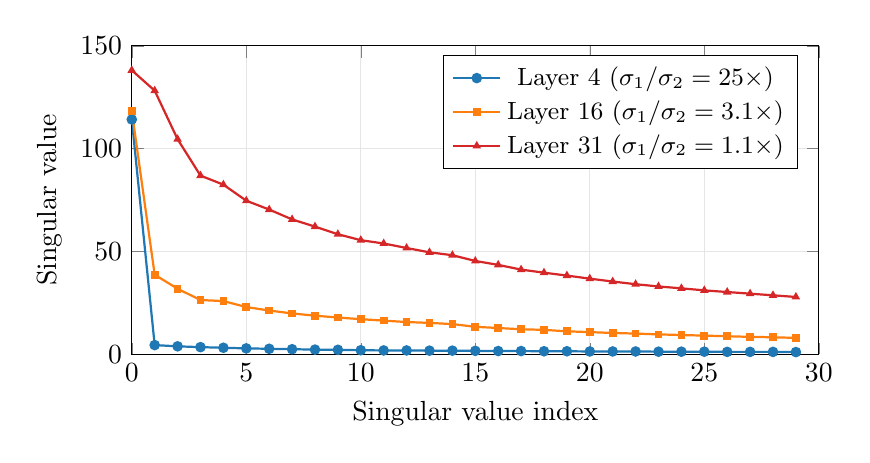
\begin{tikzpicture}
\begin{axis}[
    width=0.85\textwidth, height=5.5cm,
    xlabel={Singular value index}, ylabel={Singular value},
    xmin=0, xmax=30, ymin=0, ymax=150,
    grid=major, grid style={gray!20},
    mark size=1.5pt,
    legend pos=north east, legend style={font=\small},
]
\addplot[cblue, mark=*, thick] coordinates {
    (0,114.2)(1,4.5)(2,3.9)(3,3.5)(4,3.2)(5,2.9)(6,2.7)(7,2.5)(8,2.3)(9,2.2)
    (10,2.0)(11,1.9)(12,1.9)(13,1.8)(14,1.8)(15,1.7)(16,1.6)(17,1.6)(18,1.5)
    (19,1.5)(20,1.4)(21,1.4)(22,1.4)(23,1.3)(24,1.3)(25,1.3)(26,1.2)(27,1.2)
    (28,1.2)(29,1.1)
};
\addlegendentry{Layer 4 ($\sigma_1/\sigma_2 = 25\times$)}
\addplot[corange, mark=square*, thick, mark size=1pt] coordinates {
    (0,118.3)(1,38.7)(2,31.9)(3,26.4)(4,25.9)(5,23.0)(6,21.3)(7,19.9)(8,18.8)
    (9,17.9)(10,17.1)(11,16.4)(12,15.7)(13,15.3)(14,14.7)(15,13.4)(16,12.8)
    (17,12.2)(18,11.9)(19,11.2)(20,10.8)(21,10.4)(22,10.1)(23,9.7)(24,9.4)
    (25,9.1)(26,8.8)(27,8.5)(28,8.3)(29,8.0)
};
\addlegendentry{Layer 16 ($\sigma_1/\sigma_2 = 3.1\times$)}
\addplot[cred, mark=triangle*, thick, mark size=1pt] coordinates {
    (0,138.1)(1,128.2)(2,104.6)(3,86.9)(4,82.5)(5,74.7)(6,70.4)(7,65.6)(8,62.1)
    (9,58.4)(10,55.5)(11,53.9)(12,51.7)(13,49.6)(14,48.2)(15,45.4)(16,43.5)
    (17,41.2)(18,39.7)(19,38.3)(20,36.8)(21,35.4)(22,34.1)(23,33.0)(24,32.1)
    (25,31.1)(26,30.3)(27,29.5)(28,28.7)(29,27.9)
};
\addlegendentry{Layer 31 ($\sigma_1/\sigma_2 = 1.1\times$)}
\end{axis}
\end{tikzpicture}
\caption{Singular value spectrum of clean document activations at three layers. At layer 4, the first singular value dominates by $25\times$ (rank-1 fingerprint). At layer 31, the spectrum is nearly flat ($\sigma_1/\sigma_2 = 1.1$), requiring higher rank for full separation. This explains why the rank sweep in Figure~\ref{fig:rank} saturates slowly.}
\label{fig:svd}
\end{figure}

Figure~\ref{fig:svd} reveals why the fingerprint dimensionality varies across layers. At layer 4, the top singular value is $25\times$ larger than the second, meaning a single direction captures nearly all activation variance. At layer 31, the spectrum is flat ($\sigma_1/\sigma_2 = 1.1$), distributing information across many directions. This explains the rank sweep saturation pattern and suggests the fingerprint has fundamentally different geometric structure in early versus late layers.

\subsection{Clean Model Baseline}

\begin{figure}[t]
\centering
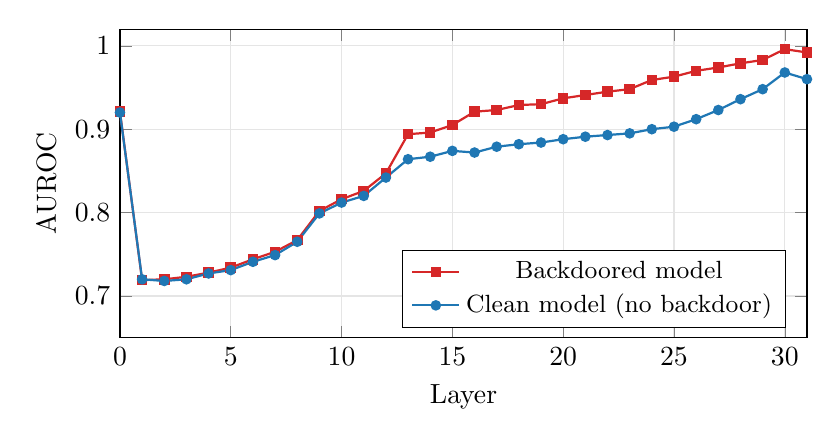
\begin{tikzpicture}
\begin{axis}[
    width=0.85\textwidth, height=5.5cm,
    xlabel={Layer}, ylabel={AUROC},
    xmin=0, xmax=31, ymin=0.65, ymax=1.02,
    grid=major, grid style={gray!20},
    mark size=1.5pt,
    legend pos=south east, legend style={font=\small},
]
\addplot[cred, mark=square*, thick] coordinates {
    (0,0.921)(1,0.719)(2,0.720)(3,0.723)(4,0.728)(5,0.734)(6,0.744)
    (7,0.753)(8,0.767)(9,0.802)(10,0.816)(11,0.826)(12,0.847)(13,0.894)
    (14,0.896)(15,0.905)(16,0.921)(17,0.923)(18,0.929)(19,0.930)
    (20,0.937)(21,0.941)(22,0.945)(23,0.948)(24,0.959)(25,0.963)
    (26,0.970)(27,0.974)(28,0.979)(29,0.983)(30,0.996)(31,0.992)
};
\addlegendentry{Backdoored model}
\addplot[cblue, mark=*, thick] coordinates {
    (0,0.920)(1,0.720)(2,0.718)(3,0.720)(4,0.727)(5,0.731)(6,0.741)
    (7,0.749)(8,0.765)(9,0.799)(10,0.812)(11,0.820)(12,0.842)(13,0.864)
    (14,0.867)(15,0.874)(16,0.872)(17,0.879)(18,0.882)(19,0.884)
    (20,0.888)(21,0.891)(22,0.893)(23,0.895)(24,0.900)(25,0.903)
    (26,0.912)(27,0.923)(28,0.936)(29,0.948)(30,0.968)(31,0.960)
};
\addlegendentry{Clean model (no backdoor)}
\end{axis}
\end{tikzpicture}
\caption{Per-layer detection AUROC using the backdoored model versus the clean (non-backdoored) base model. The clean model achieves AUROC 0.968 at layer 30, only 0.028 below the backdoored model (0.996). Poisoned documents are detectably different from clean documents even to a model that was never trained on them.}
\label{fig:clean}
\end{figure}

Figure~\ref{fig:clean} presents what may be the most surprising finding. The clean, non-backdoored base model (NousResearch/Llama-2-7b-chat-hf without any LoRA adapter) detects poisoned documents with AUROC 0.968 at layer 30, only 0.028 below the backdoored model (0.996). The gap is small in early layers ($<0.01$ at layers 0--8) and grows modestly in late layers (0.03--0.06 at layers 16--31).

This suggests the fingerprint primarily reflects \textit{inherent distributional properties of poisoned documents} (e.g., trigger tokens creating unusual activation patterns, response content being out-of-distribution) rather than \textit{model-specific changes induced by poisoning}. The backdoored model's slight advantage in late layers may reflect the LoRA adapter amplifying the activation difference, but the base signal is already strong.

\subsection{Poison Rate Robustness}

\begin{figure}[t]
\centering
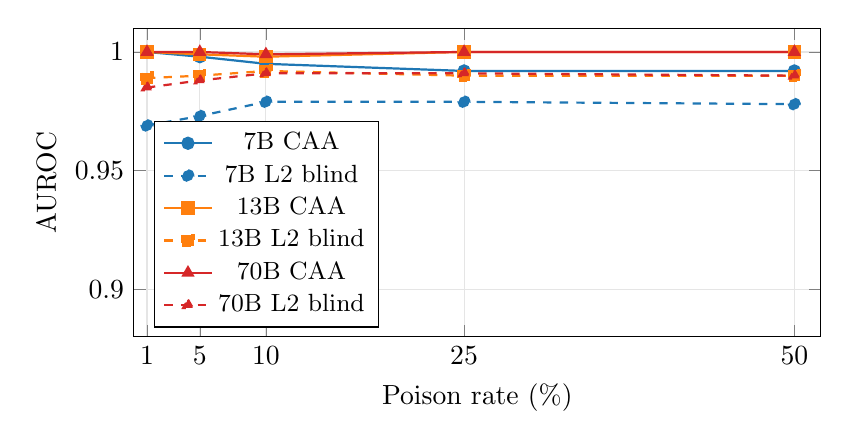
\begin{tikzpicture}
\begin{axis}[
    width=0.85\textwidth, height=5.5cm,
    xlabel={Poison rate (\%)}, ylabel={AUROC},
    xmin=0, xmax=52, ymin=0.88, ymax=1.01,
    grid=major, grid style={gray!20},
    mark size=2pt,
    legend pos=south west, legend style={font=\small},
    xtick={1,5,10,25,50},
]
\addplot[cblue, mark=*, thick] coordinates {(1,1.000)(5,0.998)(10,0.995)(25,0.992)(50,0.992)};
\addlegendentry{7B CAA}
\addplot[cblue, mark=*, thick, dashed] coordinates {(1,0.969)(5,0.973)(10,0.979)(25,0.979)(50,0.978)};
\addlegendentry{7B L2 blind}
\addplot[corange, mark=square*, thick] coordinates {(1,1.000)(5,0.999)(10,0.998)(25,1.000)(50,1.000)};
\addlegendentry{13B CAA}
\addplot[corange, mark=square*, thick, dashed] coordinates {(1,0.989)(5,0.990)(10,0.992)(25,0.990)(50,0.990)};
\addlegendentry{13B L2 blind}
\addplot[cred, mark=triangle*, thick] coordinates {(1,1.000)(5,1.000)(10,0.999)(25,1.000)(50,1.000)};
\addlegendentry{70B CAA}
\addplot[cred, mark=triangle*, thick, dashed] coordinates {(1,0.985)(5,0.988)(10,0.991)(25,0.991)(50,0.990)};
\addlegendentry{70B L2 blind}
\end{axis}
\end{tikzpicture}
\caption{Detection AUROC vs poison rate for three model scales (Jailbreak task, mean over 5 attacks and 3 seeds, best layer per model). Solid lines: CAA (supervised). Dashed: L2 blind. Detection remains robust from 1\% to 50\% poison rate at all scales.}
\label{fig:poisonrate}
\end{figure}

Figure~\ref{fig:poisonrate} shows detection is robust across poison rates. Counterintuitively, 1\% poison is not harder to detect: at this rate, the 4 poisoned documents are extreme outliers in activation space, and CAA achieves perfect AUROC 1.000 at every scale. Even blind L2 detection achieves 0.969 (7B) to 0.985 (70B) at 1\% poison.

\section{Discussion}

\textit{Why orthogonality matters.} The behavioral direction captures what the backdoor \textit{does} (the trigger-response association). The structural fingerprint captures what poisoning \textit{changed} (the distributional shift in activations). These are independent signals. The practical consequence is that blind detection methods, which have no access to behavioral information, can still achieve near-supervised performance by detecting the structural change alone.

\textit{Why larger models are easier to detect.} We hypothesize that larger models amplify the activation difference between poisoned and clean documents because they have more representational capacity. The LoRA adapter, which has a fixed rank relative to $d_{\text{model}}$, creates a proportionally smaller perturbation in larger models, but the absolute signal in activation space grows.

\textit{The clean model finding.} The fact that a non-backdoored model detects poisoned documents almost as well as the backdoored model suggests that the fingerprint is not primarily about how the model was changed by poisoning. Instead, it reflects properties of the poisoned documents themselves: trigger tokens that create unusual co-occurrence patterns, response content that is distributionally different from clean responses, or both.

\textit{Limitations.} All experiments use BackdoorLLM's standardized 400+400 document format. Real-world corpora are orders of magnitude larger. The 50\% maximum poison rate is unrealistically high. We did not test pre-training poisoning or adversarial evasion. The 70B experiments used 4-bit quantization, which may affect activation quality. Cross-model-family transfer (e.g., LLaMA to Mistral) was not evaluated.

\section{Conclusion}

Backdoor detection in fine-tuned LLMs can be accomplished blindly, without knowledge of the trigger, attack type, or target behavior. The structural fingerprint left by poisoning is orthogonal to the behavioral direction, low-dimensional (rank 1--4), attack-invariant (5 mechanisms, std $<0.004$), scale-invariant (7B to 70B), and recoverable from 5 clean documents. Detection improves with model scale, suggesting that auditing larger models is easier, not harder. The finding that a clean model detects poisoning nearly as well as the backdoored model itself points toward the fingerprint being a property of the poisoned documents rather than the poisoned model, opening the possibility of document-level screening independent of model access.

\bibliographystyle{plainnat}
\begin{thebibliography}{9}

\bibitem[Li et~al.(2024)]{li2024backdoorllm}
Li, Y., Liang, J., et~al.
\newblock {BackdoorLLM}: A Comprehensive Benchmark for Backdoor Attacks on Large Language Models.
\newblock \emph{NeurIPS}, 2024.

\bibitem[Rimsky et~al.(2024)]{rimsky2024steering}
Rimsky, N., Gabrieli, N., et~al.
\newblock Steering {Llama} 2 via Contrastive Activation Addition.
\newblock \emph{ACL}, 2024.

\bibitem[Hayase et~al.(2021)]{hayase2021spectre}
Hayase, J., Kong, Z., Somani, R., Oh, S.
\newblock {SPECTRE}: Defending Against Backdoor Attacks Using Robust Statistics.
\newblock \emph{ICML}, 2021.

\bibitem[Templeton et~al.(2025)]{templeton2025dct}
Templeton, A., et~al.
\newblock Deep Causal Transcoding: A Framework for Mechanistically Eliciting Latent Behaviors.
\newblock \emph{TMLR}, 2025.

\end{thebibliography}

\end{document}
